\documentclass{article}
\usepackage[utf8]{inputenc}
\usepackage{enumerate}
\usepackage{graphicx}
\usepackage{apacite}

\begin{document}
\begin{titlepage}
	\begin{center}
		\vspace*{1cm}
		\Huge
		\textbf{Term Paper}
		
		\vspace{0.5cm}
		Professional Software Development
		UC2PSD052
		
		\vspace{5cm}
		\textbf{Antonious Gobrial}
		
		04.12.2022
		
		
		
	\end{center}
\end{titlepage}
\tableofcontents
\thispagestyle{empty}

\newpage
\setcounter{page}{1} 
\setcounter{section}{1} 
% So that sections reflect question they answer.

\section{Requirements Engineering and System Design}
The scenario is the \textbf{\textit{bookTrainTicket}}, in the use case of an \textbf{\textit{InternationalTrainTravels}} module.
\subsection{(a) Functional requirements}
\begin{enumerate}
	\item User will be able  to sign up for an app using their personal information. Initially, this will be done via email and password.
	\item System must check that the email isn't already registered.
	\item System must notify the user of invalid inputs.
	\item Users who have created an account will be able to log in, input a destination, and view available routes to the desired location, as well as departure times.
\end{enumerate}

\subsection{(b) Non-functional requirements}
\begin{itemize}
	\item Speed is an important \underline{product requirement}. The system should have the capacity to quickly respond to user commands, and maintain up-to-date data. 
	\item Portability is an example of an \underline{organizational requirement}, defined by how the system operates in one environment compared to another. The system should be capable of running successfully on all the appropriate operating systems used by users.
	\item 2 Security is a critical \underline{external requirement}. Sensitive data must be protected to an appropriate level. Through the implementation of security features, an organization handling data should protect said data in all its states.
\end{itemize}
\newpage

\subsection{(c) Class diagram}
\begin{figure}[ht]
	\centering
	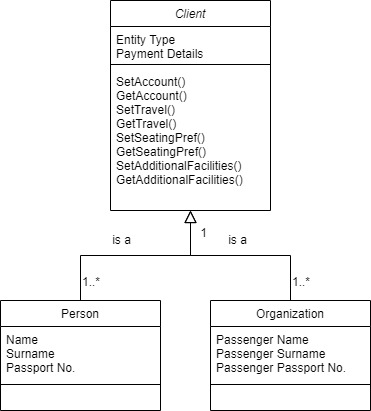
\includegraphics[scale=0.6]{2_c_class_diagram_client_person_org.jpg}
	\caption{Class diagram showing inheritance}
	\label{fig:class_diag_client_person_org}
\end{figure}
\newpage

\subsection{(d) UML and explanation for \textit{one-to-one} vs \textit{one-to-many} relationships}
In a one to one relationship, also notated as 1:1, objects are related to a maximum of one object. Figure 2 is a UML diagram showing an example of a \textit{one-to-one} relationship.
\begin{figure}[h]
	\centering
	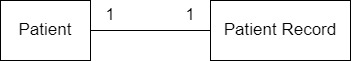
\includegraphics[scale=0.6]{2_d_1to1.jpg}
	\caption{UML 1:1 relationship}
	\label{fig:1to1relationship}
\end{figure}

In a one to many relationship, also notated as 1..*, objects can be mapped to an unlimited number of other objects. Figure 3 is a UML diagram showing an example of a \textit{one-to-many} relationship.
\begin{figure}[h]
	\centering
	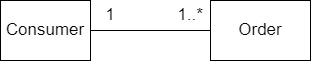
\includegraphics[scale=0.6]{2_d_1toM.jpg}
	\caption{UML 1:M relationship}
	\label{fig:1toMrelationship}
\end{figure}
\subsection{(e) Composite use-case diagram for client with five interactions}
\begin{figure}[h]
	\centering
	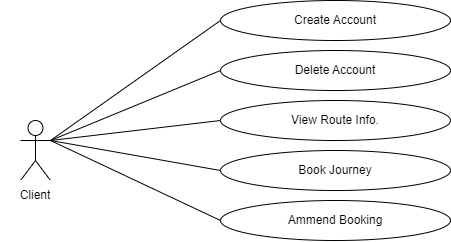
\includegraphics[scale=0.6]{2_e_use_case_diagram_client.jpg}
	\caption{Use-case diagram for client}
	\label{fig:use_case_client}
	\end{figure}
\newpage
\subsection{(f) UML for \textit{bookTrainTicket}}
\begin{figure}[h]
	\centering
	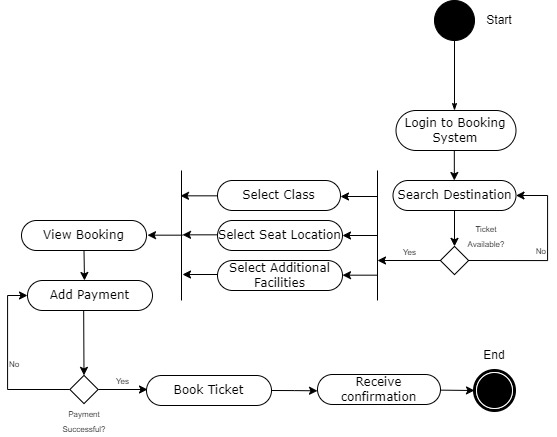
\includegraphics[scale=0.6]{2_f_UML_bookTrainTicket.jpg}
	\caption{UML diagram for \textbf{\textit{bookTrainTicket}}}
	\label{fig:UML_bookTrainTicket}
\end{figure}
\newpage
\subsection{(g) Sequence diagram depicting client logging into booking system portal}
\begin{flushleft}
Sequence diagrams are used to show the flow of messages. These are either inputs from actors, or outputs from the objects contained within a system. The message will always have a direction - arrows are used to indicate where the message was initiated, and its destination.
\end{flushleft}
\begin{figure}[h]
	\centering
	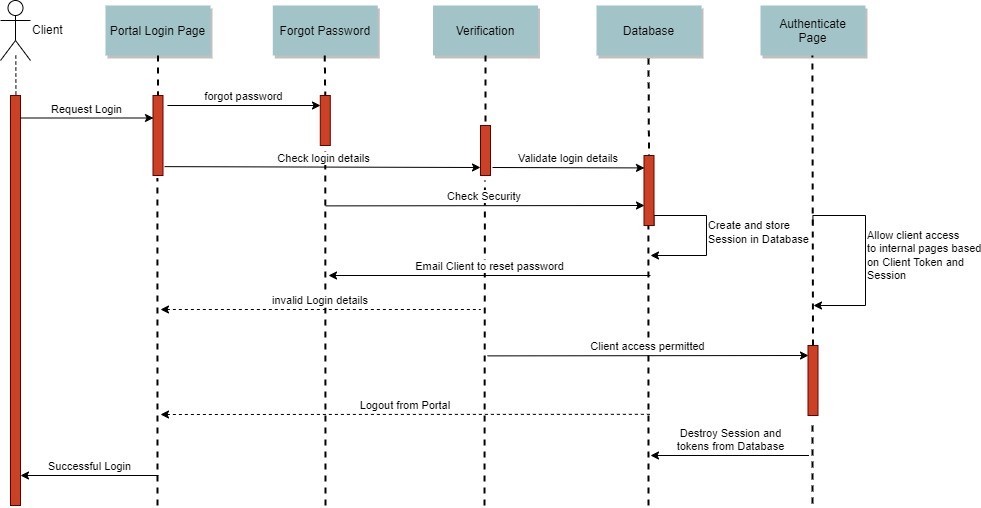
\includegraphics[width=\columnwidth]{2_g_sequence_diagram_login.jpg}
	\caption{Sequence diagram for booking system portal}
	\label{fig:Seq_booking_system_portal}
\end{figure}

\newpage
\section{Software Testing Methodologies}
\subsection{(a) Scenario Testing}
\begin{enumerate}
	\item \textbf{Scenario:} On weekdays, Greg travels to and from his job, in a neighbouring city. His day starts with a 15 minute walk to the train station, then a hour train journey, followed by another 15 minute walk to reach his office. For 5 years Greg has purchased his train ticket at the train station. However, recently there have been many train cancellations which results in Greg being late for work. Greg has decided he needs to know if the train service is operating, before he leaves his home. Greg has decided its best to download and install the Booking app, so he can make sure he's never late for work again.
		\subitem \textbf{Test Case 1}
		\subitem Objectives: Retrieve up-to-date train information
		\subitem Pre-requisites: Live booking system, good internet connection. 
		\subitem Test Data: Search of desired destination, from current location.
		\subitem Test Steps: Input destination, Input time of travel, click on search.
		\subitem Expected Results: Journey displayed with correct start and end points, at the correct time of day.
		\subitem \textbf{Test Case 2}
		\subitem Objectives: Notify client of delayed or cancelled service.
		\subitem Pre-requisites: Live booking system, good internet connection, push messages to client permitted, client saves a service to be notified about if it is delayed or cancelled. 
		\subitem Test Data: Services affected by delay or cancellation, push notification to clients using these services.
		\subitem Test Steps: Update service, notify client.
		\subitem Expected Results: Customer receives a message when the service they use is affected.
		\newline
	\item \textbf{Scenario:} Greg has now installed the app which allows him to book his train to and from work. He has viewed his regular train and saved it as a favourite. He isn't sure whether he wants to pay for the monthly or annual pass but will just pay for his tickets individually. He is also unsure which card to use, so he will decide that when he is purchasing each ticket.
		\subitem \textbf{Test Case 1}
		\subitem Objectives: Payment is successful.
		\subitem Pre-requisites: Valid card, chosen a valid ticket.
		\subitem Test Data: Card details, payment verification and receipt.
		\subitem Test Steps: Fill in card details, click on purchase.
		\subitem Expected Results: Client gets confirmation of booking and payment, client receives a payment receipt.
		\subitem \textbf{Test Case 2}
		\subitem Objectives: Payment is unsuccessful.
		\subitem Pre-requisites: Payment card which doesn't pass approval, chosen a valid ticket.
		\subitem Test Data: Card details, payment declined message, method to trigger next attempt.
		\subitem Test Steps: Fill in card details, click on purchase.
		\subitem Expected Results: Client receives message of unsuccessful payment, and given the option of another attempt, max 3 attempts.
		\newline
	\item \textbf{Scenario:} Greg has been happily using the Booking system for a few months now, so he decides to buy his weeks worth of tickets, on the weekend before. But Greg falls sick on a Monday afternoon and is sent home, his boss tells him to take the rest of the week off. Greg wants to cancel the remaining tickets for that week and get a refund.
		\subitem \textbf{Test Case 1}
		\subitem Objectives: Cancel tickets and get a refund.
		\subitem Pre-requisites: Tickets are refundable, tickets are not within 24 hours of departure time.
		\subitem Test Data: Booking details, payment details.
		\subitem Test Steps:View booking, cancel booking, receive cancellation confirmation, receive refund.
		\subitem Expected Results: Client is able to cancel ticket(s) and will receive a refund to the payment method used.
		\subitem \textbf{Test Case 2}
		\subitem Objectives: Cancel tickets without a refund.
		\subitem Pre-requisites: Tickets are within 24 hours of departure.
		\subitem Test Data: Booking details, payment details.
		\subitem Test Steps: View booking, confirm cancellation without refund, cancel booking, receive cancellation confirmation.
		\subitem Expected Results: Client is able to cancel ticket(s) upon confirming they won't get a refund.
		\newline
	\item \textbf{Scenario:} Greg has been doing well in his job and has received a promotion. However, this means will be travelling alot more. On any given day, he will travel to multiple locations. He doesn't know more than a few days in advance so he will be booking his tickets as he needs them.
		\subitem \textbf{Test Case 1}
		\subitem Objectives: Client books multiple tickets at the same time
		\subitem Pre-requisites: Journey start can be edited, multiple tickets can be added to a basket before purchase.
		\subitem Test Data: Live booking system, good internet connection, shopping basket.
		\subitem Test Steps: Client inputs start and end point of a journey, selects ticket, adds ticket to basket, repeats process several times.
		\subitem Expected Results: Client creates a basket with multiple tickets that snake around the country, and performs one payment action.
		\subitem \textbf{Test Case 2}
		\subitem Objectives: Client is warned of booking a ticket which intersects the journey time of another ticket, when attempting to add it to the basket.
		\subitem Pre-requisites: Basket object is operational, ticket travel time clashes with another tickets travel time.
		\subitem Test Data: Live booking system, good internet connection, shopping basket, compare current booking to those in the basket.
		\subitem Test Steps: Client inputs start and end point of a journey, selects ticket, attempts to add ticket to basket, receives warning that ticket clashes with another ticket in the basket, ammends ticket, adds ticket to basket.
		\subitem Expected Results: Client is warned when attempting to add a ticket which clashes with an existing ticket in the basket. The client can decide whether to continue with adding the ticket to the basket, or to ammend first.
\end{enumerate}
\subsection{(b) 2 validation and 2 defective test that can be performed on AC}
\subsubsection{Validation testing}
\begin{enumerate}
	\item Check if the AC unit is able to reduce the temperature of a room during summer.
	\item Check if the AC unit is able to increase the temperature of a room during winter.
\end{enumerate}
\subsubsection{Defective testing}
\begin{enumerate}
	\item Check the performance of an AC unit when the coolant level is brought to below the recommended level.
	\item Check the performance of an AC unit when the airflow is restricted. Starting at a low restriction, increment towards complete restriction to test for performance of the system as well as error handling carried out by the system to detect such an issue.
\end{enumerate}
\subsubsection{Assumptions}
\begin{itemize}
	\item The room is insulated to common building standards, as well as checked that no drafts are present. 
	\item The installation of the unit was carried out by a professional.
	\item The GUI of the AC will display a temperature, but for comparison, the room temperature should be measured independently of the system.
	\item The coolant system has no leaks, and the unit is otherwise under normal operation.
	\item The components involved in air circulation, are all functioning correctly.
\end{itemize}
\subsection{(c) Difference between unit testing, component testing and system testing}
\begin{flushleft}
The three stages of development testing are \textit{unit testing, component testing,} and \textit{system testing}. All these testing methods are involved in finding defects or bugs in software \cite{sommerville2016software}.
\end{flushleft}
\begin{itemize}
	\item \textbf{Unit testing} is where the functionality of an individual program unit is tested. An example of unit testing would be isolating part of the login system software, to test the code which checks if an email address is already registered to a client, and how it handles errors.
	\item \textbf{Component testing} is also a type of software testing, however it concerns the usability of each individual component. Components may be entities such as object classes or functions; or even groups of these entities. An example of component testing, to refer to the train booking system, would be to test how data flows between the components of the system which are involved in returning the correct price of a ticket once a client has selected it.
	\item \textbf{System testing} is the testing of the integration of an entire system. It is concerned with showing that a system meets functional and non-functional requirements, as well as testing system properties. This is often a multi-stage process, the subsystems are tested before the integrated system is tested \cite{sommerville2016software}. An example of system testing, would be performance testing a car prototype that has been manufactured. Initially the components of the car will have undergone unit testing - to establish if each component is functioning as intended, as well as component testing - how subsystems come together and that they perform as expected. The integration of these subsystems creates the final product i.e. the car. The car will then be tested for performance, reliability, crash-testing and so on. This is system testing.
\end{itemize}

\newpage
\section{Software Development Life Cycle}
\subsection{(a) Waterfall vs Agile}
\begin{flushleft}The pros and cons of the \textbf{waterfall method} are as follows:\end{flushleft}
\begin{flushleft}
	Pros:
\end{flushleft}
\begin{itemize}
	\item Pre-defined objectives result in effective use of time to complete tasks.
	\item Timescales are pre-defined and kept, to ensure efficiency.
	\item Testing is simplified using this model.
	\item The output is accurate as per the requirement.
\end{itemize}
Cons:
\begin{itemize}
	\item Difficulty faced when defining the proper needs.
	\item Lack of flexibility.
	\item Requires the most time for the delivery of the product.
	\newline
\end{itemize}
\begin{flushleft}
	The pros and cons of the \textbf{Agile method} are as follows:
\end{flushleft}
\begin{flushleft}
	Pros:
\end{flushleft}
\begin{itemize}
	\item Responds very well to changing objectives.
	\item Accepts uncertainty.
	\item Has faster review cycles.
	\item Highly flexible in releasing features.	
\end{itemize}
Cons:
\begin{itemize}
	\item Moves forward with a lack of complete understanding of the problem.
	\item More flexibility can lead to poor behaviour or performance.
	\item Lacks predictability.
\end{itemize}
\begin{flushleft}
	The main difference between the waterfall and the agile methods, can be summed up as follows: the waterfall method is a linear life cycle approach, whereas the agile method is a continuous iteration approach to development and testing in the software development life cycle. The agile method allows more flexibility but in the waterfall their is an structured methodology of the software development.
\end{flushleft}

\subsection{(b) Project where Spiral Development Life Cycle Model is preferred over Validation and Verification Life Cycle Model}
\begin{flushleft}
	The spiral model, also referred to as the evolutionary process model, was pioneered by Barry Boehm as an incremental and cyclical approach to the development process. The key factor which makes the spiral model different from other software process models is its explicit recognition of risk. Risk is simply what can go wrong.  Each loop is divided into 4 sectors \cite{sommerville2016software}:
\begin{itemize}
	\item Objective setting
	\item Risk assessment reduction
	\item Development and validation
	\item Planning 
\end{itemize} 
	The validation and verification life cycle model (V-model) is made up of its two subcategories: validation testing, and verification testing. Beginning with verification testing, it is the process of analysing predetermined software specifications. These include documents, code, design and programs - to ensure the product meets these specifications. The tester develops a product by carrying out the following activities:
\begin{itemize}
	\item Identifying business requirements
	\item Identifying system requirements
	\item Design Review
	\item Code walkthrough
\end{itemize}
	Validation testing, also referred to as dynamic testing, entails functional and non-functional testing. It is the process of ensuring that products satisfy the intended purpose, set out by the client. Functional tests include:
\begin{itemize}
	\item Unit testing
	\item Integration testing
	\item System testing
\end{itemize}
Non-functional testing includes:
\begin{itemize}
	\item User acceptance testing
\end{itemize}
	Take for example the creation of a new software application like a booking system for a train service. The benefit of a spiral model is that it will allow for the creation of a functional application relatively quickly, so that it can be launched. The same application, developed using the V-model, will require more time before launch due to rigidity in the case of utilization, and a lack of flexibility in terms of design - the V-model by definition doesn't suit projects that aim to release early prototypes.
\newline
\newline
	It is also appropriate to use the spiral model, as it is designed for projects where systems are divided into subsystems that can be developed incrementally, while allowing the core features to remain operational. In this case, requirements are expected to evolve over time, and the application must handle updates while operational to some degree. This renders the V-model unsuitable as it is not designed for small scale updates, rather it is suited for large updates which result in the application being offline.
\end{flushleft}
\newpage
\section{Version Control}
\subsection{(a) 4 reasons for a version control system}
\begin{enumerate}
	\item Keeping track of changes - who made them, and when they made them.
	\item Allowing collaboration between multiple developers
	\item Facilitating backups and increasing productivity vs manual version control.
	\item Bug fixes are shared - ensures maintenance of different software versions.
\end{enumerate}
\subsection{(b) Centralized (CVCS) vs Distributed (DVCS) version control systems}
\subsubsection{3 advantages of DVCS over CVCS}
\begin{enumerate}
	\item Code base is distributed therefore doesn't have a single point of failure.
	\item Branching allows the system to overcome slow network connections.
	\item For large team collaboration, CVCS has difficulty finding stable moments to push changes. Hence, DVCS has greater stability.
\end{enumerate}
\subsubsection{Examples of centralized and distributed version control systems}
\begin{itemize}
	\item Subversion (SVN) is an example of a CVCS.
	\item Git is an example of a DVCS.
\end{itemize}
\subsection{(c) Branching in version control systems}
\subsubsection{What is branching?}
\begin{flushleft}
	Branching allows developers to work on code at the same time, without duplicating effort. A branch is a copy of a codeline, managed by a version control system \cite{zolkifli2018version}.
\end{flushleft}
\subsubsection{3 uses of branching}
\begin{enumerate}
	\item Physical branching: branches created for files, components and subsystems.
	\item Functional branching: branches of a systems functional configuration - created for features, logical changes and any unit of deliverable functionality.
	\item Organizational branching: branches of a teams work effort - created for groups, roles, tasks and subprojects \cite{appleton1998streamed}.
\end{enumerate}
\section{Working with Git}
\subsection{(a) Random integer generator}
\begin{figure}[ht]
	\centering
	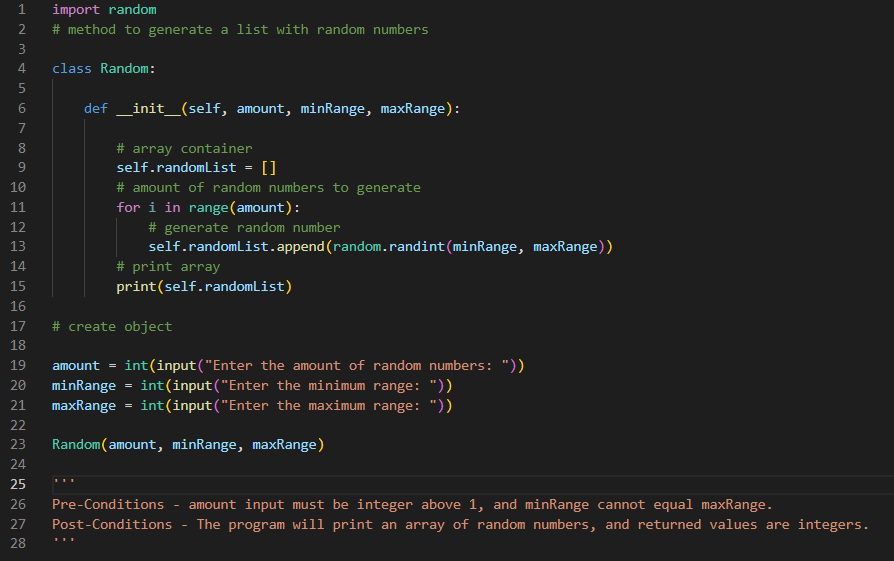
\includegraphics[width=\textwidth]{6_a_random_int_gen.png}
	\caption{Screenshot of Random integer generator}
	\label{fig:random_int_gen}
\end{figure}
\newpage
\subsection{(b) Updating the project 3 times by adding appropriate commit message before updating the existing version}
Figure 8 shows the \textit{Git Bash} script for committing the python file to the \textbf{staging area}.
\begin{figure}[ht]
	\centering
	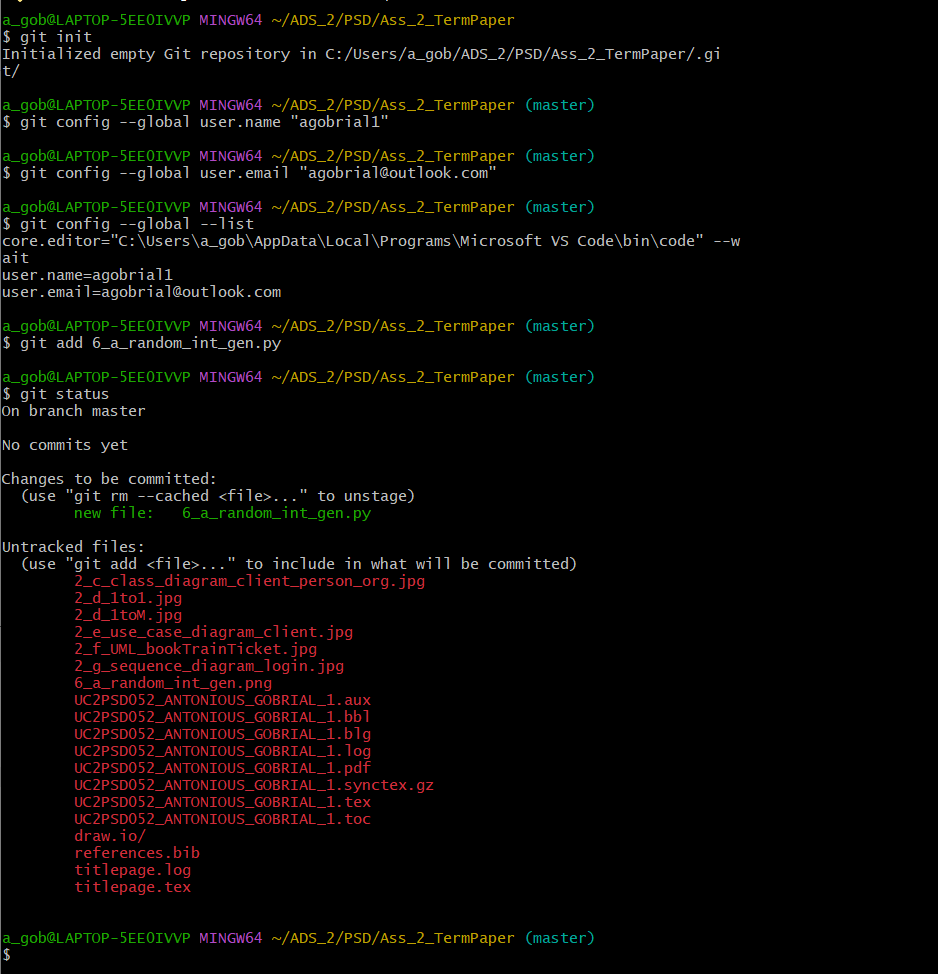
\includegraphics[width=\textwidth]{git_1.png}
	\caption{Committing file to the Staging area}
	\label{fig:git_1}
\end{figure}
\newpage
The following figures show how the file was committed to the repository.
\begin{figure}[ht]
 	\centering
 	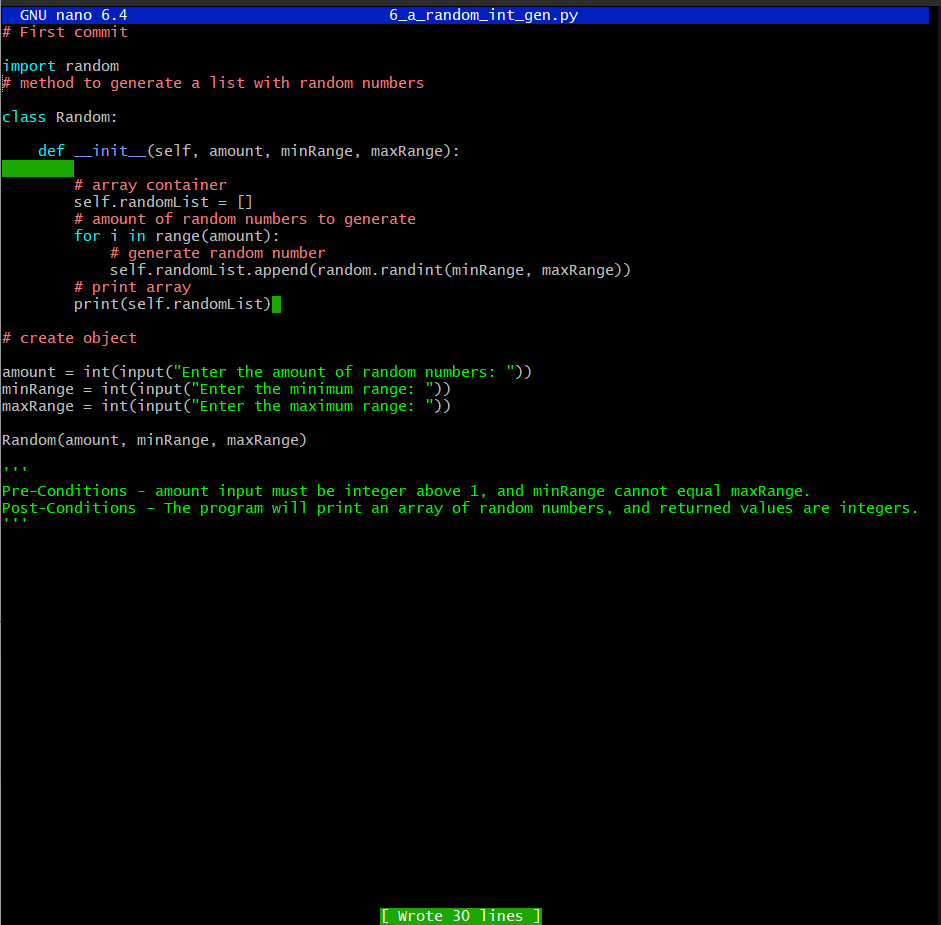
\includegraphics[width=\textwidth]{git_2.png}
 	\caption{Commenting first modification on the file}
 	\label{fig:git_2}
\end{figure}
 \begin{figure}[ht]
	\centering
	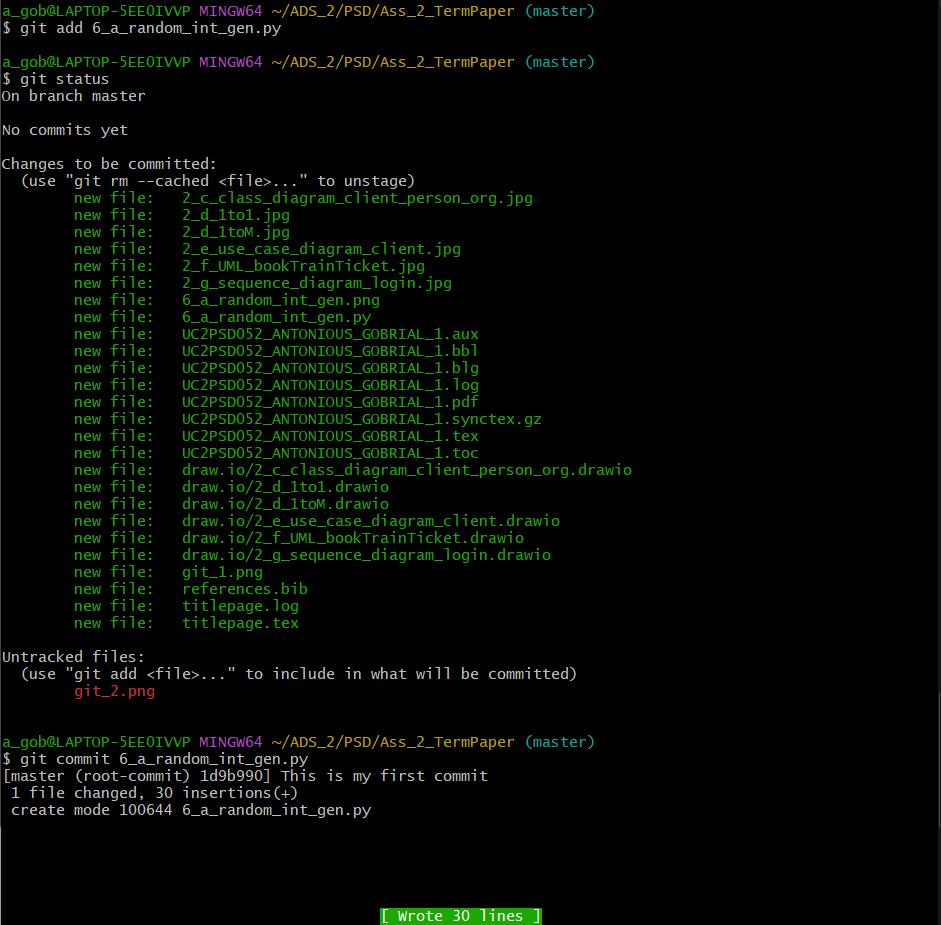
\includegraphics[width=\textwidth]{git_3.png}
	\caption{Committing to repository}
	\label{fig:git_3}
\end{figure}
\begin{figure}[ht]
	\centering
	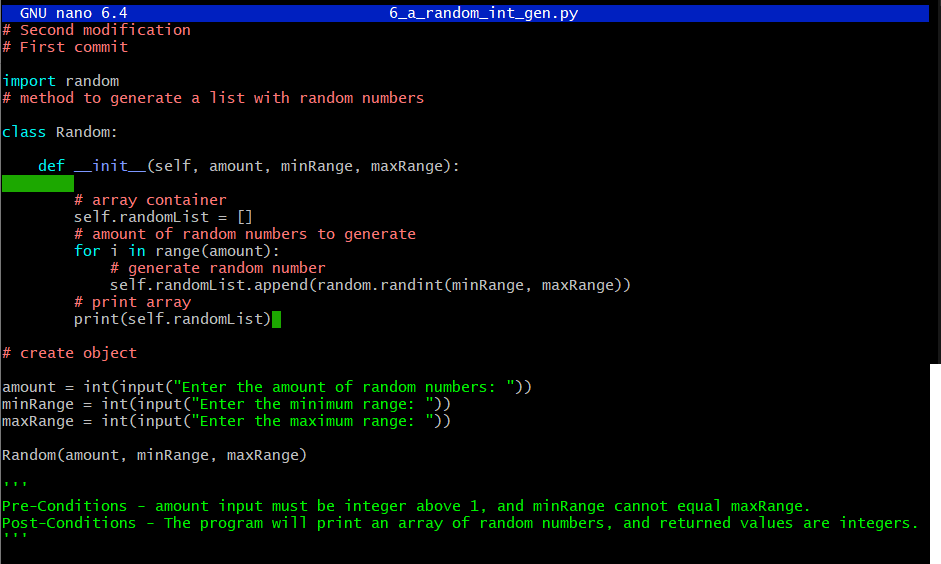
\includegraphics[width=\textwidth]{git_4.png}
	\caption{Second modification}
	\label{fig:git_4}
\end{figure}

\newpage
\bibliographystyle{apacite}
\bibliography{references.bib}
\end{document}